\documentclass[conference]{IEEEtran}

% -----------------------------------------------------------------------------
% Core packages
% -----------------------------------------------------------------------------
\usepackage{cite}
\usepackage{amsmath,amssymb,amsfonts}
\usepackage{graphicx}
\usepackage{booktabs}
\usepackage{multirow}
\usepackage{textcomp}
\usepackage{xcolor}
\usepackage{url}
\usepackage[hidelinks]{hyperref}
\usepackage{tikz}
\usetikzlibrary{positioning, arrows.meta, calc}

% Figures are stored in paper/figures/.
\graphicspath{{figures/}}

% BibTeX logo.
\def\BibTeX{{\rm B\kern-.05em{\sc i\kern-.025em b}\kern-.08em
    T\kern-.1667em\lower.7ex\hbox{E}\kern-.125emX}}

\begin{document}

% -----------------------------------------------------------------------------
% Title and authors
% -----------------------------------------------------------------------------
\title{Training-Free Image Cosegmentation with Foundation Model Features and Spectral Analysis}

% TODO: Replace the placeholders below with the final author list and
% affiliations. Add additional \and blocks as needed.
\author{
\IEEEauthorblockN{Lucas Lattari}
\IEEEauthorblockA{
\textit{Instituto Federal do Sudeste de Minas Gerais}\\
Rio Pomba, Brazil
}
\and
\IEEEauthorblockN{Second Author}
\IEEEauthorblockA{
\textit{Department or Institution}\\
City, Country
}
}

\maketitle

% -----------------------------------------------------------------------------
% Abstract and keywords
% -----------------------------------------------------------------------------
\begin{abstract}
% TODO: Write the abstract after the main contributions and experimental
% results have stabilized. A useful structure is:
% context/problem -> gap -> proposed approach -> main results -> conclusion.
This extended manuscript presents an image co-segmentation framework.
The abstract will be completed as the manuscript and experimental analysis
are consolidated.
\end{abstract}

\begin{IEEEkeywords}
image co-segmentation, computer vision, self-supervised learning,
visual representations, spectral methods, foundation models
\end{IEEEkeywords}

% -----------------------------------------------------------------------------
% Main text
% -----------------------------------------------------------------------------
\section{Introduction}
\input{sections/01_introduction}

\section{Related Work}
\input{sections/02_related_work}

\section{Proposed Method}
\subsection{Method Overview}

The problem is defined as follows. Consider an image collection $\mathcal{I} = {I_1, \dots, I_n}$ belonging to the same class. Our goal is to produce a set of binary segmentation masks $\mathcal{M} = {M_1, \dots, M_n}$ that identifies the common foreground across the collection. We assume that each image $I_i$ contains a visually consistent common foreground.

The proposed method differs from single-image segmentation, since the computation of each segmentation mask is based on the entire image collection $\mathcal{I}$. Moreover, it follows a training-free approach: no stage of the pipeline is trained or fine-tuned specifically for cosegmentation. All pretrained components are used as provided, without task-specific adaptation.

Our hypothesis is that patches belonging to the common foreground tend to present similar visual semantics among the images in the collection. These similarities can be used to compute cross-image correspondences. However, recurring background patterns introduce an additional challenge, since visually similar regions may also be shared by multiple images. Because of that, our method combines semantic patch representations, cross-image correspondence structure, spectral graph analysis, recurring-background suppression, spatial priors, and foundation-model-based mask refinement.

Initially, we extract patch features using DINOv2~\cite{oquab2023dinov2} (stage E1). We then select similar image pairs and, for each pair, construct a joint patch-affinity graph that is partitioned using Normalized Cuts~\cite{shi2000normalized}. The resulting pairwise foreground decisions are aggregated into correspondence scores for each patch (stage E2). After NCut, we suppress evidence associated with recurring background patterns (stage E2B). Stage E3 performs global spectral clustering over the entire image collection and combines the resulting patch clusters with correspondence and spatial evidence to produce a coarse foreground mask for each image. Stage E4 employs SAM2~\cite{ravi2024sam2}, a foundation model for promptable visual segmentation, to convert coarse co-saliency estimates into spatially precise object masks. Finally, stage E5 iteratively refines the masks until convergence. Fig.~\ref{fig:pipeline} depicts the entire pipeline.
\begin{figure*}[t]
\centering

\resizebox{0.98\textwidth}{!}{%
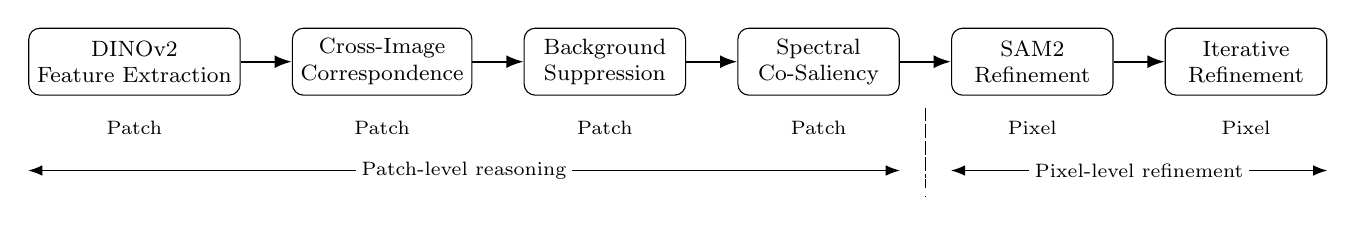
\begin{tikzpicture}[
    node distance=0.65cm,
    block/.style={
        draw,
        rounded corners,
        align=center,
        font=\footnotesize,
        minimum width=2.05cm,
        minimum height=0.85cm,
        inner sep=3pt
    },
    arrow/.style={
        -{Latex[length=2.2mm]},
        thick
    },
    level/.style={
        font=\scriptsize
    },
    stagebar/.style={
        {Latex[length=1.8mm]}-{Latex[length=1.8mm]},
        thin
    }
]

% -------------------------------------------------------------------------
% Pipeline stages
% -------------------------------------------------------------------------

\node[block] (e1)
    {DINOv2\\Feature Extraction};

\node[block, right=of e1] (e2)
    {Cross-Image\\Correspondence};

\node[block, right=of e2] (e2b)
    {Background\\Suppression};

\node[block, right=of e2b] (e3)
    {Spectral\\Co-Saliency};

\node[block, right=of e3] (e4)
    {SAM2\\Refinement};

\node[block, right=of e4] (e5)
    {Iterative\\Refinement};


% -------------------------------------------------------------------------
% Pipeline arrows
% -------------------------------------------------------------------------

\draw[arrow] (e1) -- (e2);
\draw[arrow] (e2) -- (e2b);
\draw[arrow] (e2b) -- (e3);
\draw[arrow] (e3) -- (e4);
\draw[arrow] (e4) -- (e5);


% -------------------------------------------------------------------------
% Processing granularity
% -------------------------------------------------------------------------

\node[level, below=0.20cm of e1]  (l1) {Patch};
\node[level, below=0.20cm of e2]  (l2) {Patch};
\node[level, below=0.20cm of e2b] (l2b) {Patch};
\node[level, below=0.20cm of e3]  (l3) {Patch};
\node[level, below=0.20cm of e4]  (l4) {Pixel};
\node[level, below=0.20cm of e5]  (l5) {Pixel};


% -------------------------------------------------------------------------
% Conceptual processing levels
% -------------------------------------------------------------------------

\draw[stagebar]
    ([yshift=-0.95cm]e1.south west)
    --
    node[
        midway,
        fill=white,
        inner sep=2pt,
        font=\scriptsize
    ] {Patch-level reasoning}
    ([yshift=-0.95cm]e3.south east);

\draw[stagebar]
    ([yshift=-0.95cm]e4.south west)
    --
    node[
        midway,
        fill=white,
        inner sep=2pt,
        font=\scriptsize
    ] {Pixel-level refinement}
    ([yshift=-0.95cm]e5.south east);

\draw[dashed, thin]
    ($(e3.south east)!0.5!(e4.south west)+(0,-0.22)$)
    --
    ($(e3.south east)!0.5!(e4.south west)+(0,-1.28)$);


% -------------------------------------------------------------------------
% Granularity transition marker
% -------------------------------------------------------------------------

\draw[dashed, thin]
    ($(e3.south east)!0.5!(e4.south west)+(0,-0.15)$)
    --
    ($(e3.south east)!0.5!(e4.south west)+(0,-1.05)$);

\end{tikzpicture}%
}

\caption{
Overview of the proposed training-free image co-segmentation pipeline.
The first stages perform collection-level reasoning at patch granularity,
using self-supervised features, cross-image correspondences, recurring-background
suppression, and spectral co-saliency analysis.
The resulting coarse foreground estimates are subsequently converted into
pixel-level masks through SAM2-based refinement and iterative mask refinement.
}
\label{fig:pipeline}

\end{figure*}

The following subsections describe each component of the proposed framework in detail.

\subsection{Self-Supervised Patch Feature Extraction}

Object cosegmentation requires identifying semantically corresponding
foreground regions across images despite variations in appearance, pose,
scale, viewpoint, illumination, and spatial
location~\cite{rubinstein2013unsupervised, bristow2015dense}. Handcrafted
descriptors such as SIFT and HOG offer some geometric and photometric
invariance, but this is not inherently semantic and may be insufficient
under large intra-class variation~\cite{bristow2015dense,
kim2017fcss}. Self-supervised Vision Transformer features, in contrast,
encode spatially localized semantic information and have proven
effective as dense descriptors for zero-shot semantic correspondence and
object cosegmentation~\cite{oquab2024dinov2,amir2023effectiveness}.

Stage E1 converts each image into a spatial grid of self-supervised
DINOv2 descriptors~\cite{oquab2024dinov2}; no cross-image reasoning is
performed here, and the resulting descriptors constitute the shared
representation consumed by all later stages. Given a collection
$\mathcal{I}=\{I_1,\dots,I_n\}$, each image is encoded by a frozen
ViT-S/14 backbone $\Phi$, which operates on non-overlapping
$14\times14$-pixel patches and outputs one descriptor per patch, plus a
global class token. For image $I_i$, this yields a patch-token grid of
$H_p \times W_p = P$ patches, with $\mathbf{f}_i^{(u)} \in
\mathbb{R}^D$ ($D=384$; see Sec.~\ref{sec:ablation-backbone}) denoting
the descriptor of patch $u \in \{1,\dots,P\}$, stacked into
\begin{equation}
\mathbf{F}_i =
\begin{bmatrix} \mathbf{f}_i^{(1)} \\ \vdots \\ \mathbf{f}_i^{(P)} \end{bmatrix}
\in \mathbb{R}^{P \times D},
\end{equation}
together with a global class token $\mathbf{c}_i \in \mathbb{R}^D$,
retained for image-level use in Sec.~\ref{sec:e2}. Descriptors are taken
from the last transformer block with the backbone's final layer
normalisation applied
\footnote{Via \texttt{get\_intermediate\_layers(n=1,
return\_class\_token=True)}, which applies this normalisation by
default.} — the representation exposed by DINOv2's own frozen-feature
evaluation protocol. Earlier blocks or attention-key facets have been
reported preferable for semantic correspondence in prior
work~\cite{amir2023effectiveness}; we do not ablate this axis, so results
in Sec.~\ref{sec:results} reflect the backbone as released.

\subsubsection{Aspect-Ratio-Preserving Encoding}

The global patch graph of Sec.~\ref{sec:e3} connects patches across
images, which requires a fixed token count $P$ for every image and
therefore a common input resolution. Resizing anisotropically to
$S\times S$ would satisfy this but distort object shape. We instead
resize isotropically so the longest side matches $S$, then pad to a
square canvas with per-channel ImageNet means (less disruptive to a
pretrained backbone than black/white padding). With $S=518=37\times 14$,
every image yields a $37\times 37$ grid, $P=1369$. This preserves aspect
ratio at the cost of introducing content-free patches.

\subsubsection{Valid-Patch Bookkeeping}

For each image, E1 persists the rescaling geometry
$(h_i', w_i', \delta_i^{\text{top}}, \delta_i^{\text{left}})$, from which
later stages derive a validity mask $\mathcal{V}_i$: a patch is retained
if its extent overlaps the rescaled image region, so only patches lying
entirely within the padding margins are discarded. Because all images
share the same constant-colour padding, fully padded patches are
near-identical within and across images and would otherwise register as
the most consistently repeated content in the collection — a systematic
false positive under any recurrence-based foreground criterion. Boundary
patches straddling the content border still encode real structure and
are kept. Invalid patches are removed as nodes from the sparse global
patch graph (Sec.~\ref{sec:e3}), rather than zeroed, since zeroed but
present nodes would still contribute to degree statistics and Laplacian
normalisation and could absorb one of the $K$ spectral clusters. The same
mask excludes invalid patches from the pairwise foreground voting of
Sec.~\ref{sec:e2}, and predicted masks are cropped to the content region
before evaluation.

Patch and class-token descriptors are $\ell_2$-normalised before being
written to disk, so that inner products reduce to cosine similarity,
bounded in $[-1,1]$ and comparable across images and collections — this
also keeps the softmax temperature of Sec.~\ref{sec:e2} on a consistent
scale, independent of each patch's raw activation strength.

Feature extraction runs once per collection, with no stochastic
component (inference mode, no augmentation, no gradient), and persists
descriptors together with patch-grid dimensions, original image sizes,
and rescaling geometry, so patch indices can always be mapped back to
pixel coordinates. All later ablations therefore read from identical
descriptors, isolating each stage's contribution. Unless stated
otherwise, all experiments use ViT-S/14 at $S=518$ with
aspect-ratio-preserving encoding and $\ell_2$-normalised descriptors
(Table~\ref{tab:production-defaults} lists the full set of calibrated
defaults for every stage).

The patch grid also lower-bounds the spatial detail E1 can represent:
each token summarises a $14\times14$ region of the padded canvas
(\textasciitilde$13.5\times13.5$ px of the original image for iCoseg,
whose images are rarely larger than $500$ px on the longest side, so
rescaling discards no pixel information). Elongated structures narrower
than this extent — limbs, poles, cables — are not resolved by any single
descriptor and cannot be recovered by the refinement stages of
Sec.~\ref{sec:e4}--\ref{sec:e5}, which adjust boundaries but inherit the
coarse foreground estimate from patch-level reasoning. This is a
distinct failure mode from the merging of nearby object instances, which
originates in the correspondence and clustering stages rather than in
the representation (Sec.~\ref{sec:limitations} discusses both, and a
preliminary multi-scale feature fusion experiment aimed at the former).

\subsection{Cross-Image Correspondence Graph Construction}
\label{sec:e2}

\subsubsection{Degree-Based Affinity Reweighting}

\subsection{Recurring-Background Suppression}

\subsection{Spectral Co-Saliency Estimation}

\subsubsection{Adaptive Empty-Foreground Recovery}

Foreground-orientation and graph construction retain any patch overlapping the content region, whereas the recovery mechanism and the background model of Sec.~\ref{sec:e2b} require the patch centre to fall inside it. The stricter criterion excludes boundary patches that are predominantly padding, whose descriptors are constant across the collection; both mechanisms select patches by similarity to a reference set, and are therefore sensitive to that degeneracy in a way that graph partitioning is not.

\subsection{Foundation Model-Based Mask Refinement}

\subsubsection{Initial SAM2 Refinement}

\subsubsection{Iterative Mask Refinement}

\section{Experimental Setup}
\begin{table}[t]
\centering
\caption{Calibrated production defaults per pipeline stage. CLI defaults in individual scripts differ where noted; \texttt{run\_pipeline.sh} overrides them with the values below.}
\label{tab:production-defaults}
\begin{tabular}{@{}llll@{}}
\toprule
\textbf{Stage} & \textbf{Hyperparameter} & \textbf{Value} & \textbf{Ref.} \\
\midrule
\multirow{4}{*}{E1 --- Feature extraction}
  & Backbone            & ViT-S/14 (\texttt{dinov2\_vits14}) & \ref{sec:ablation-backbone} \\
  & Input size $S$      & 518 ($37\times14$)                 & \S\ref{sec:e1} \\
  & Resize mode         & \texttt{keep\_ar}                  & \S\ref{sec:e1} \\
  & Feature mode        & \texttt{l2} ($\ell_2$-normalised)  & \S\ref{sec:e1} \\
\midrule
\multirow{4}{*}{E2 --- Correspondence}
  & \texttt{top\_k}         & 60     & \ref{sec:ablation-e2} \\
  & Temperature          & 0.05   & \ref{sec:ablation-e2} \\
  & Orientation           & \texttt{spatial}   & \ref{sec:ablation-e2} \\
  & Degree reweighting $\alpha$ & 0.10 & \ref{sec:ablation-e2} \\
\midrule
\multirow{3}{*}{E2B --- Background suppression}
  & Mode                & \texttt{recurrence} & \ref{sec:ablation-e2b} \\
  & $\lambda$            & 0.50               & \ref{sec:ablation-e2b} \\
  & $\gamma$             & 0.00               & \ref{sec:ablation-e2b} \\
\midrule
\multirow{3}{*}{E3 --- Co-saliency}
  & Clusters $K$         & 8      & \ref{sec:ablation-e3} \\
  & $k$-NN neighbours    & 15     & \ref{sec:ablation-e3} \\
  & Saliency $\alpha$    & 0.5    & \ref{sec:ablation-e3} \\
\midrule
\multirow{3}{*}{E4 --- SAM refinement}
  & Model                & SAM~2.1 Hiera-Large & \ref{sec:ablation-e4} \\
  & Prompt mode          & \texttt{box\_points\_mask} & \ref{sec:ablation-e4} \\
  & Iterations           & 2      & \ref{sec:ablation-e4} \\
\midrule
\multirow{4}{*}{E5 --- Iterative refinement}
  & Max. iterations      & 20     & \ref{sec:ablation-e5} \\
  & Convergence threshold & 0.99  & \ref{sec:ablation-e5} \\
  & FG seed points       & 8      & \ref{sec:ablation-e5} \\
  & BG seed points       & 8      & \ref{sec:ablation-e5} \\
\bottomrule
\end{tabular}
\end{table}

\section{Results}
\section{Results}
\label{sec:results}

We evaluate our training-free co-segmentation pipeline on iCoseg \cite{batra2010icoseg} and PASCAL-VOC CoSeg \cite{everingham2010pascal, faktor2013}, following the evaluation protocols described in Section~\ref{sec:experimental-setup}. We report both pixel-level accuracy\footnote{Faktor and Irani~\cite{faktor2013} and the subsequent literature following their protocol report this quantity as ``Precision'' (P); their stated definition -- the percentage of pixels correctly classified as either foreground or background -- is identical to standard pixel accuracy $(TP+TN)/N$, where $N = TP+TN+FP+FN$ is the total pixel count, not to the classification-theoretic precision $TP/(TP+FP)$. We verified this equivalence directly from their protocol description and adopt the more standard \emph{accuracy} terminology throughout, using P and Acc.\ interchangeably when referencing their reported numbers.} and Jaccard index (IoU), the two metrics most consistently used across the co-segmentation literature, allowing direct comparison with prior work.

We first compare our method against prior work under directly comparable protocols (Section~\ref{sec:comparison}). We then analyze per-class performance to characterize where the pipeline succeeds and where it struggles (Section~\ref{sec:per-class}), present qualitative results that illustrate the progression of the pipeline's intermediate stages (Section~\ref{sec:qualitative}), and examine representative failure modes (Section~\ref{sec:failure-analysis}).

\subsection{Comparison with Previous Methods}
\label{sec:comparison}

Direct comparison across co-segmentation methods is complicated by the lack of a single standardized evaluation protocol: prior work reports results on different subsets of iCoseg (ranging from 8 to 38 class groups), different image-pairing schemes for PASCAL-VOC, and inconsistent conventions for what counts as a standard benchmark. To avoid the misleading comparisons that this heterogeneity invites, we restrict the tables below to results obtained under protocols that are directly compatible with ours: the full iCoseg set of 38 groups / 643 images (Section~\ref{sec:results-icoseg}), and the 1{,}037-image / 20-class PASCAL-VOC~2010 co-segmentation protocol introduced by Faktor and Irani~\cite{faktor2013} (Section~\ref{sec:results-pascal}). Methods evaluated under incompatible protocols (e.g., the 16-class iCoseg subset used in several earlier works) are excluded from the main tables; where relevant, we discuss them qualitatively rather than reporting misaligned numbers side by side.

Among prior work, Faktor and Irani~\cite{faktor2013} and Hsu et al.~\cite{hsu2018} are particularly relevant points of comparison: both report results on the full 38-class / 643-image iCoseg dataset and on the same 1{,}037-image / 20-class PASCAL-VOC~2010 split, making their numbers directly comparable to ours under matching protocols. Hsu et al.~\cite{hsu2018} represent the strongest unsupervised baseline under these protocols, using an end-to-end trainable co-attention CNN built on ImageNet-pretrained ResNet-50 features -- a substantially different paradigm from both the classical composition-based approach of~\cite{faktor2013} and our own training-free use of frozen foundation-model features (DINOv2, SAM2). Notably, while Hsu et al.\ do not rely on human-annotated masks, their method still performs a per-collection gradient-based optimization (60 epochs per image set) to fit the co-attention generator network -- unlike our pipeline, which applies no learned or optimized component specific to the co-segmentation task at any stage.

Perhaps the most methodologically relevant prior work is Amir et al.~\cite{amir2022deepvit}, who similarly adopt a training-free approach, applying lightweight clustering directly to dense features extracted from a frozen, self-supervised Vision Transformer (DINO-ViT) -- the direct predecessor of the DINOv2 backbone used in our pipeline. On the same PASCAL-VOC protocol, their zero-shot method already performs on par with the unsupervised-but-trained CNN of Hsu et al.~\cite{hsu2018} in Jaccard index (0.607 vs.\ 0.60, a marginal 0.007 gap), suggesting that frozen self-supervised features were already competitive with task-specific training prior to the availability of DINOv2 and SAM2. Our result reinforces this parity rather than resolving it in either direction: at 90.78\% accuracy and 0.5975 IoU, our pipeline sits almost exactly between Amir et al.'s DINO-ViT figures (88.2\%/0.607) and Hsu et al.'s trained CNN (91.0\%/0.60) in accuracy, while our IoU falls marginally below both (by 0.0095 and 0.0025, respectively). In other words, moving from DINO-ViT to DINOv2 features and adding SAM2-based mask refinement preserves the competitiveness of frozen self-supervised features established by Amir et al., but does not translate into a clear improvement over their training-free baseline on this particular protocol -- unlike the pattern on iCoseg (Section~\ref{sec:results-icoseg}), where our pipeline is essentially on par with the mask-supervised RL-CoSeg refinement stage. Notably, Amir et al.\ do not report results on iCoseg, so this comparison is limited to the PASCAL-VOC table.

Between these two poles of supervision, Wang et al.~\cite{wang2017nparitite} occupy an intermediate position: they use a fine-tuned fully convolutional network (FCN) to generate semantically informed candidate regions, but the core co-segmentation mechanism -- discovering multiple co-occurring matching cliques over an augmented N-partite graph via mixed-binary integer programming -- remains an unsupervised combinatorial procedure with no task-specific training. Despite this partial reliance on a trained component, their iCoseg result (93.8\%/0.77) is essentially matched by our fully training-free pipeline (94.23\%/0.7734), while on PASCAL-VOC our result (90.78\%/0.5975) clearly exceeds theirs (84.3\%/0.522) by 6.48 accuracy points and 0.0755 IoU (14.5\% relative). This suggests that the semantic proposal generation Wang et al.\ obtain from a fine-tuned FCN provides little advantage over frozen foundation-model features on the harder, more cluttered PASCAL-VOC protocol.

On the full iCoseg dataset, we additionally compare against Duan et al.~\cite{duan2022rlcoseg} (RL-CoSeg), which reports a competitive Precision/Jaccard of 94.2\%/0.78. This comparison, however, requires a caveat regarding supervision: unlike the unsupervised or training-free methods above, RL-CoSeg trains an actor-critic reinforcement learning network on ground-truth-annotated image pairs from PASCAL VOC~2012 and MSRC, and applies it as a boundary-refinement stage on top of the initial segmentation produced by a separate co-segmentation network~\cite{gong2020} -- itself a supervised Siamese network trained on the same annotated datasets. Its reported number therefore reflects two successive mask-supervised stages rather than an end-to-end unsupervised or training-free pipeline. Despite this substantially more favorable supervision setting, our training-free result (94.23\%/0.7734) is essentially on par with theirs, which we view as a meaningful data point for the central claim of this paper: that frozen foundation-model features, without any task-specific training or fine-tuning, can match methods that rely on mask-level supervision at every stage.

Finally, we report the recent transformer-based UFGS method of Su et al.~\cite{su2024ufgs}, which unifies co-segmentation, co-saliency detection, and video salient object detection under a single architecture and achieves the strongest numbers on both benchmarks among all methods considered here (98.1\%/0.923 on iCoseg, 96.9\%/0.757 on PASCAL-VOC). This result requires the strongest supervision caveat of the comparisons in this section: UFGS is trained end-to-end on COCO-SEG, a dataset of 200{,}000 mask-annotated images spanning 78 groups, using a combination of classification, weighted binary cross-entropy, and IoU losses. Its performance therefore reflects the benefit of large-scale mask supervision rather than the zero-shot or unsupervised setting shared by the other methods in Tables~\ref{tab:icoseg38-comparison} and~\ref{tab:pascal-comparison}, including ours. This result establishes UFGS as an approximate ceiling for what large-scale mask supervision can achieve on these benchmarks, rather than a peer for direct comparison with the training-free methods above -- the gap in supervision cost is simply too large for the comparison to be methodologically fair. Framed differently, however, the gap between UFGS and our result quantifies the price of forgoing that supervision: 3.87 accuracy points and 0.150 IoU on iCoseg (19.4\% relative), widening to 6.12 accuracy points and 0.160 IoU on PASCAL-VOC (26.7\% relative). Our pipeline requires no annotated data, no training run, and no fine-tuning to close most of this gap, whereas UFGS depends on 200,000 manually annotated masks and roughly 20 hours of dedicated training. We view this trade-off, rather than the raw ranking implied by Tables~\ref{tab:icoseg38-comparison} and~\ref{tab:pascal-comparison}, as the more informative reading of this comparison.

\subsubsection{Results on iCoseg-38}
\label{sec:results-icoseg}

Table~\ref{tab:icoseg38-comparison} compares our pipeline against five prior methods on the full iCoseg-38 protocol (38 groups, 643 images), spanning the supervision spectrum introduced in Section~\ref{sec:comparison}.

\begin{table}[t]
\centering
\caption{Comparison on the full iCoseg dataset (38 groups / 643 images).}
\label{tab:icoseg38-comparison}
\begin{tabular}{lccccc}
\toprule
Method & Year & Supervision & External model & Acc.\ / P$^\dagger$ (\%) & IoU / J \\
\midrule
Faktor \& Irani~\cite{faktor2013} & 2013 & Unsupervised & -- & 92.8 & 0.73 \\
Wang et al.~\cite{wang2017nparitite} & 2017 & Semantic proposals + unsupervised matching$^\ddagger$ & FCN & 93.8 & 0.77 \\
Duan et al.\ (RL-CoSeg)~\cite{duan2022rlcoseg} & 2022 & Supervised (mask-trained refinement) & ResNet-50 + A3C RL & 94.2 & 0.78 \\
Hsu et al.~\cite{hsu2018} & 2018 & Unsupervised & CNN (ResNet-50) & 96.5 & 0.84 \\
Su et al.\ (UFGS)~\cite{su2024ufgs} & 2024 & Supervised (COCO-SEG, mask-trained) & VGG16 + Transformer & 98.1 & 0.923 \\
\textbf{Ours} & 2026 & \textbf{Training-free} & \textbf{DINOv2 + SAM2} & \textbf{94.23} & \textbf{0.7734} \\
\bottomrule
\end{tabular}
\vspace{2pt}
\footnotesize{$^\dagger$P here denotes the pixel accuracy of Faktor and Irani~\cite{faktor2013}; see Section~\ref{sec:results} for the equivalence with our accuracy metric. $^\ddagger$Wang et al.\ use an FCN fine-tuned on a 3{,}480-image subset of VOC Context for generic semantic candidate generation, but perform co-occurrence discovery via an unsupervised graph-matching formulation (N-partite graph, mixed-binary integer program) with no task-specific training for co-segmentation.}
\end{table}

Faktor and Irani's classical, training-free approach~\cite{faktor2013} offers a particularly informative point of contrast, since it shares the defining characteristic of our pipeline -- no task-specific training of any kind -- while relying on a fundamentally different generation of visual representation. Their method composes co-segments from hand-crafted HOG and color-histogram descriptors, scored via a statistical-significance criterion over randomly sampled region matches; ours replaces this with dense patch features from a frozen, self-supervised vision transformer (DINOv2), followed by spectral co-saliency estimation and SAM2-based mask refinement. Despite neither method involving any learned, task-specific component, our result exceeds theirs by 1.43 accuracy points and 0.0434 IoU (5.9\% relative).

This gap is best read not as a claim that our pipeline is a better-engineered instance of the same idea, but as evidence that the underlying visual representation itself has improved substantially in the decade separating the two methods. HOG and color histograms encode local gradient and color statistics with no semantic grounding; DINOv2 features, by contrast, emerge from large-scale self-supervised pretraining and encode high-level object and part semantics directly in their patch-level representation~\cite{oquab2024dinov2}. The comparison therefore isolates, in a controlled way, how much of the gap to fully supervised methods (Hsu et al.~\cite{hsu2018}, Su et al.~\cite{su2024ufgs}) can be closed by upgrading the representation alone, without introducing any task-specific supervision.

Across the full comparison, our pipeline (94.23\%/0.7734) sits just above the classical training-free baseline (92.8\%/0.73), essentially matches the partially-trained methods (93.8--94.2\%/0.77--0.78; Wang et al.~\cite{wang2017nparitite}, Duan et al.~\cite{duan2022rlcoseg}), and trails only the two fully supervised, end-to-end trained networks (96.5--98.1\%/0.84--0.923; Hsu et al.~\cite{hsu2018}, Su et al.~\cite{su2024ufgs}). Positioned this way, the full iCoseg-38 comparison offers concrete support for this paper's central argument: frozen foundation-model features move training-free co-segmentation substantially closer to what task-specific supervision achieves, even as a residual gap to the most heavily supervised methods persists.

\subsubsection{Results on PASCAL-VOC CoSeg-1037}
\label{sec:results-pascal}

Table~\ref{tab:pascal-comparison} compares our pipeline against five prior methods on the 1{,}037-image, 20-class PASCAL-VOC 2010 protocol introduced by Faktor and Irani~\cite{faktor2013}, spanning the same supervision spectrum as Table~\ref{tab:icoseg38-comparison}.
\begin{table}[t]
\centering
\caption{Comparison on PASCAL-VOC 2010 co-segmentation (20 classes / 1{,}037 images, protocol of~\cite{faktor2013}).}
\label{tab:pascal-comparison}
\begin{tabular}{lccccc}
\toprule
Method & Year & Supervision & External model & Acc.\ / P$^\dagger$ (\%) & IoU / J \\
\midrule
Faktor \& Irani~\cite{faktor2013} & 2013 & Unsupervised & -- & 84.0 & 0.46 \\
Wang et al.~\cite{wang2017nparitite} & 2017 & Semantic proposals + unsupervised matching$^\ddagger$ & FCN & 84.3 & 0.522 \\
Amir et al.~\cite{amir2022deepvit} & 2022 & \textbf{Training-free} & DINO-ViT & 88.2 & 0.607 \\
Hsu et al.~\cite{hsu2018} & 2018 & Unsupervised & CNN (ResNet-50) & 91.0 & 0.60 \\
Su et al.\ (UFGS)~\cite{su2024ufgs} & 2024 & Supervised (COCO-SEG, mask-trained) & VGG16 + Transformer & 96.9 & 0.757 \\
\textbf{Ours} & 2026 & \textbf{Training-free} & \textbf{DINOv2 + SAM2} & \textbf{90.78} & \textbf{0.5975} \\
\bottomrule
\end{tabular}
\vspace{2pt}
\footnotesize{$^\dagger$P here denotes the pixel accuracy of Faktor and Irani~\cite{faktor2013}; see Section~\ref{sec:results} for the equivalence with our accuracy metric. $^\ddagger$Wang et al.\ use an FCN fine-tuned on a 3{,}480-image subset of VOC Context for generic semantic candidate generation, but perform co-occurrence discovery via an unsupervised graph-matching formulation with no task-specific training for co-segmentation.}
\end{table}

With the full-dataset run now complete, we can compare the PASCAL-VOC result directly against the iCoseg-38 result in Table~\ref{tab:icoseg38-comparison}. Our pipeline achieves 90.78\% accuracy and 0.5975 IoU on PASCAL-VOC CoSeg-1037, against 94.23\%/0.7734 on iCoseg-38 -- a drop of 3.45 accuracy points (3.7\% relative) and 0.176 IoU points (22.7\% relative). This mirrors, though does not reach the severity of, the pattern already documented by Faktor and Irani~\cite{faktor2013}, whose Jaccard index falls from 0.73 on iCoseg to 0.46 on PASCAL-VOC (a 37\% relative drop). As with their method, the smaller relative drop in accuracy compared to IoU is consistent with PASCAL-VOC's background-dominated images -- the authors report background occupying over 90\% of pixels in many PASCAL images -- since accuracy, dominated by the (correctly predicted) background class, is far less sensitive to this shift than IoU, which directly penalizes imprecise foreground boundaries. The per-class breakdown (Section~\ref{sec:per-class}) shows this degradation is concentrated in a handful of classes with small, thin, or heavily cluttered objects -- chair (IoU 0.257), pottedplant (0.236), diningtable (0.267), and person (0.351) -- while classes with large, visually distinct objects such as bus (0.930), cow (0.838), and horse (0.828) remain close to iCoseg-level performance.

Across this comparison, our pipeline (90.78\%/0.5975) sits well above the classical training-free baseline (84.0\%/0.46) and the partially-trained Wang et al.~\cite{wang2017nparitite} (84.3\%/0.522), sits close to the two other training-free or lightly-supervised methods (88.2--91.0\%/0.60--0.607; Amir et al.~\cite{amir2022deepvit}, Hsu et al.~\cite{hsu2018}), and trails only the fully supervised Su et al.~\cite{su2024ufgs} (96.9\%/0.757). Unlike on iCoseg-38, where our result matched or approached most partially- and fully-trained baselines, the PASCAL-VOC protocol's smaller, more cluttered foreground objects widen the gap to supervised methods -- consistent with the per-class degradation discussed above. We discuss representative failures from this set in Section~\ref{sec:per-class-pascal}.

\subsection{Per-Class Performance Analysis}
\label{sec:per-class}

While the aggregate iCoseg-38 numbers reported in Table~\ref{tab:icoseg38-comparison} (94.23\%/0.7734) summarize overall performance, they obscure substantial variation across the 38 constituent groups: per-class IoU ranges from 0.169 to 0.982, with a standard deviation of 0.206 around a mean of 0.773. This section examines that variation to identify where the pipeline succeeds, where it struggles, and whether the failure modes are systematic enough to warrant discussion beyond the aggregate.

\subsubsection{iCoseg-38}
\label{sec:per-class-icoseg}

\paragraph{Precision, not recall, drives IoU variance -- though the source of low precision is not uniform.} Across the 38 groups, per-class IoU correlates strongly with precision ($r=0.978$) and more weakly with recall ($r=0.813$), indicating that aggregate IoU loss is driven primarily by excess predicted foreground rather than by missed objects. This pattern is consistent with over-segmentation (the shared object is found, but surrounded by extra predicted area), and several low-IoU groups fit this description cleanly (e.g., Airshows-helicopter: precision 0.560, recall 0.994). However, per-image inspection of the Airshows subgroups (Table~\ref{tab:icoseg38-lowest-groups}, marked $^\dagger$) shows that low class-level precision can also arise from a different, more severe pattern -- a mix of images with no correct detection at all alongside images that succeed normally -- which produces a similarly low aggregate precision without any single image actually exhibiting over-segmentation. The two patterns are indistinguishable from class-level aggregates alone; per-image breakdown is necessary to tell them apart. The two ``balanced/mixed'' groups in Table~\ref{tab:icoseg38-lowest-groups} (Windmill, Kite-Brighton) illustrate this limitation directly: Airshows-planes, confirmed bimodal by per-image inspection, has a gap ($-0.139$) that falls just inside this same ``balanced/mixed'' threshold, meaning the heuristic cannot rule out the same bimodal pattern for these two groups without further inspection, which we leave to future work.
\begin{table}[t]
\centering
\caption{The ten lowest-IoU groups on iCoseg-38, with failure signature inferred from the precision-recall gap (over-segmentation: gap $<-0.15$; under-segmentation: gap $>0.15$; balanced/mixed: otherwise). Only the Airshows subgroups (marked $^\dagger$) were further inspected at the per-image level (Section~\ref{sec:per-class-icoseg}, above); signatures for the remaining groups reflect class-level aggregates only.}
\label{tab:icoseg38-lowest-groups}
\begin{tabular}{lccccl}
\toprule
Group & $n$ & IoU & Prec. & Rec. & Signature \\
\midrule
Airshows-planes$^\dagger$        & 39 & 0.169 & 0.180 & 0.319 & Bimodal (61.5\% total miss) \\
Airshows-Huntsville$^\dagger$    & 22 & 0.232 & 0.232 & 0.702 & Bimodal (27.3\% total miss) \\
Gymnastics-1                     &  6 & 0.446 & 0.456 & 0.757 & Over-segmentation \\
Taj Mahal (Inde du Nord)         &  5 & 0.446 & 0.457 & 0.616 & Over-segmentation \\
Windmill                         & 18 & 0.532 & 0.552 & 0.535 & Balanced / mixed \\
Airshows-helicopter$^\dagger$    & 12 & 0.556 & 0.560 & 0.994 & Over-segmentation (confirmed) \\
Liverpool FC Players             & 33 & 0.604 & 0.649 & 0.811 & Over-segmentation \\
Woman Soccer (white)             & 16 & 0.609 & 0.653 & 0.922 & Over-segmentation \\
Kite-Brighton                    & 18 & 0.619 & 0.688 & 0.726 & Balanced / mixed \\
Monks                            & 17 & 0.634 & 0.834 & 0.665 & Under-segmentation \\
\bottomrule
\end{tabular}
\end{table}

\paragraph{The five strongest groups are both accurate and consistent.} The five highest-IoU groups are Kite-Margate (0.982), Kendo-EKC (0.973), Kite-kitekid (0.969), Gymnastics-3 (0.968), and Ferrari 599 GTB Fiorano (0.964). Unlike the weakest groups, these are not merely high on average: all five also have among the lowest within-group IoU spread in the dataset (iou\_std between 0.004 and 0.026, versus a dataset-wide mean of 0.184), indicating uniformly strong performance across every image in the group rather than a high mean masking a mix of successes and failures. This is consistent with the dataset-wide pattern already noted: within-class IoU variance correlates negatively with mean IoU ($r=-0.711$ across all 38 groups), meaning the pipeline's failures tend to be inconsistent while its successes tend to be uniform. Notably, two of the five strongest groups (Kite-Margate, Kite-kitekid) share the same open-sky backdrop implicated in the Airshows failures below -- yet the same root category also contains two markedly weaker subgroups under similar conditions (Kite-Colt Park: 0.841; Kite-Brighton: 0.619), echoing the intra-family heterogeneity already discussed. This suggests that sky alone is not sufficient to determine success or failure. Object size offers a partial explanation: across these four Kite subgroups together with the three Airshows subgroups, foreground-to-image area ratio correlates strongly with IoU ($r=0.818$, $n=7$), and the within-Kite-family correlation alone is comparable ($r=0.793$). However, object size does not fully account for the pattern: Kite-Colt Park and Airshows-helicopter have nearly identical foreground area (8.3\% and 8.9\% of the image, respectively) yet differ in IoU by 0.285 (0.841 vs.\ 0.556). We tested whether foreground-background color contrast (mean RGB Euclidean distance between the object and a sky-region proxy) explains this residual gap; it does not -- the two groups have nearly identical contrast (209.1 vs.\ 212.9), and contrast correlates \emph{negatively} with IoU across all seven groups considered ($r=-0.576$), the opposite of the hypothesized direction. This may reflect a limitation of RGB Euclidean distance as a contrast proxy (it conflates brightness and hue) rather than a genuine absence of a contrast effect, but with the evidence available, color contrast does not explain the residual gap. We leave isolating the remaining factor -- potentially the specific visual signature of aircraft versus kites, or a perceptually-calibrated color-difference metric -- to future work.

\paragraph{The Airshows groups are the pipeline's weakest case, through two distinct failure modes.} All three Airshows subgroups fall among the ten lowest-IoU groups in the dataset (Table~\ref{tab:icoseg38-lowest-groups}). Per-image inspection reveals that this aggregate conceals two qualitatively different failure patterns rather than one: in Airshows-planes, 24 of 39 images (61.5\%) are total misses (zero intersection with ground truth), and in Huntsville, 6 of 22 (27.3\%); Airshows-helicopter, by contrast, has zero total misses, and instead follows the pure over-segmentation pattern described above (recall consistently near 1.0, precision as low as 0.17). Across the 73 images in the three subgroups, the color variance inside false-positive regions is lower than inside the true foreground region in 63 cases (86.3\%) -- most consistently in Airshows-helicopter (12/12), somewhat less so in planes (35/39) and Huntsville (16/22) -- consistent with false positives being predominantly drawn from large, visually uniform background structure rather than from generic image noise, though not exclusively so.

Direct inspection of representative images (Figure~\ref{fig:airshows-failure-modes}) supports a refined version of the sky-recurrence hypothesis: rather than flat sky specifically, the shared factor appears to be large, visually salient background structure -- cloud formations, haze bands, or smoke trails -- that occupies far more image area than the aircraft themselves and, in at least one verified case, directly dominates the spectral clustering stage's saliency ranking: in image \texttt{2624969059}, two clusters together covering 89.8\% of the image were assigned foreground status, with the higher-scoring of the two (score 0.606, the second-highest of all eleven clusters in the group) corresponding to the sunlit cloud region -- while every cluster occupying under 8\% of the image, the size range in which the aircraft itself falls, was excluded from the foreground set. A second Huntsville case (image \texttt{2625770634}) was manually verified at the pixel level: despite predicted and ground-truth masks appearing visually close in the diff overlay, direct comparison at matching resolution confirmed zero true-positive overlap, ruling out an evaluation alignment artifact. E2B's effect on this pattern is inconsistent across subgroups: mean patch-level foreground likelihood decreases after background suppression in Airshows-planes and Airshows-helicopter (as intended), but \emph{increases} on average in Huntsville, indicating that background suppression does not reliably identify the dominant recurring structure in every subgroup. We do not treat this as evidence that E2B is miscalibrated in general -- it was validated on the full iCoseg-38 set (Section~\ref{sec:e2b}) -- but as a subgroup-specific interaction worth flagging as a limitation (Section~\ref{sec:limitations}) rather than a global failure of the mechanism.
\begin{figure}[t]
\centering
\begin{subfigure}[b]{0.32\linewidth}
    \centering
    \includegraphics[height=3.2cm,width=\linewidth,keepaspectratio]{figures/airshows_cloud_dominant.png}
    \caption{}
    \label{fig:airshows-cloud}
\end{subfigure}
\hfill
\begin{subfigure}[b]{0.32\linewidth}
    \centering
    \includegraphics[height=3.2cm,width=\linewidth,keepaspectratio]{figures/airshows_oversegmentation.png}
    \caption{}
    \label{fig:airshows-overseg}
\end{subfigure}
\hfill
\begin{subfigure}[b]{0.32\linewidth}
    \centering
    \includegraphics[height=3.2cm,width=\linewidth,keepaspectratio]{figures/airshows_verified_miss.png}
    \caption{}
    \label{fig:airshows-miss}
\end{subfigure}
\caption{Representative Airshows failure cases (TP=green, FP=red, FN=blue). (a) A large salient cloud formation (Huntsville, image \texttt{2624969059}) is segmented as the shared object while the aircraft, occupying under 1\% of image area, remains unmarked. (b) A correctly-localized helicopter (Airshows-helicopter, image \texttt{2803733769}) with a large adjoining false-positive region against uniform sky, illustrating the over-segmentation pattern. (c) The total-miss case (Huntsville, image \texttt{2625770634}); pixel-level comparison against ground truth confirmed zero overlap at matching resolution (Section~\ref{sec:per-class-icoseg}).}
\label{fig:airshows-failure-modes}
\end{figure}

\paragraph{Intra-family variance supports the no-override policy.} Several iCoseg root categories are split into multiple original subgroups, and the variance within a single root category is often as large as the variance across the entire dataset. Gymnastics ranges from IoU 0.446 (subgroup 1) to 0.968 (subgroup 3), a spread of 0.522; Kite ranges from 0.619 to 0.982 (spread 0.363); Taj Mahal ranges from 0.446 to 0.692 (spread 0.246). By contrast, Kendo, Pandas, Stonehenge, and Skating -- root categories with comparably sized subgroups -- show spreads of only 0.02--0.03. Notably, Gymnastics, Kite, and Taj Mahal are among the six classes used for E3 hyperparameter calibration (Section~\ref{sec:e3-graph}), yet their subgroups disagree with each other by half a point of IoU or more. This is direct evidence against per-class hyperparameter tuning: no single configuration tuned to "Gymnastics" as a category could simultaneously suit both its near-perfect subgroup (0.968) and its worst subgroup (0.446), since the source of difficulty lies in individual image characteristics rather than in any property shared by the category label itself. This reinforces the dual-criterion policy adopted throughout this work (Section~\ref{sec:experimental-setup}): configuration choices are validated against mean improvement and the absence of catastrophic degradation on any individual class, never against per-class optimality.

\subsubsection{PASCAL-VOC CoSeg-1037}
\label{sec:per-class-pascal}

\paragraph{The precision-driven pattern replicates on PASCAL-VOC, but with more class-specific heterogeneity than on iCoseg.} Across the 20 PASCAL classes, per-class IoU again correlates strongly with precision ($r=0.954$) and, more closely than on iCoseg, with recall as well ($r=0.851$ vs.\ $0.813$ on iCoseg) -- confirming that excess predicted foreground remains the dominant driver of IoU loss on this protocol too, though recall plays a comparatively larger role than on iCoseg. This aggregate pattern, however, masks class-specific heterogeneity in \emph{which} failure signature dominates: among the four lowest-IoU classes named in Section~\ref{sec:results-pascal}, diningtable (precision 0.309, recall 0.688, gap $-0.379$) and person (precision 0.399, recall 0.596, gap $-0.198$) fit the over-segmentation pattern cleanly, while chair shows both precision and recall low with no dominant direction (gap $-0.018$), and pottedplant is the sole exception with the \emph{opposite} signature -- recall lower than precision (gap $+0.050$), consistent with under-segmentation (the object is frequently missed) rather than background over-inclusion. A previously unremarked fifth low-IoU class, bicycle (IoU 0.343, gap $-0.366$), also fits the over-segmentation pattern and ranks between diningtable and person. The following per-image analysis examines whether this aggregate asymmetry reflects a single graded failure mode or, as found in the iCoseg Airshows groups, a mixture of qualitatively distinct ones.

\paragraph{Extreme classes.} The five lowest-IoU classes are pottedplant (0.236), chair (0.257), diningtable (0.267), bicycle (0.343), and person (0.351); the five highest are bus (0.930), cow (0.838), horse (0.828), car (0.795), and motorbike (0.787). The weakest classes share small, thin, or frequently occluded objects photographed against cluttered indoor or urban scenes, while the strongest involve large, texturally distinct animals or vehicles typically photographed with the object filling a substantial fraction of the frame -- consistent with the object-size and clutter-based explanation already offered in Section~\ref{sec:results-pascal}.

\paragraph{The bimodal failure pattern from Airshows generalizes to PASCAL-VOC, selectively.} Per-image data confirms that the total-miss/success bimodal pattern identified in Airshows-planes also appears in a subset of the weakest PASCAL classes, but not uniformly across all of them. Pottedplant and chair exhibit the same bimodal signature: 36.6\% (15/41) and 33.3\% (16/48) of their images, respectively, are total misses (zero intersection with ground truth), with the remaining images achieving substantially higher IoU (0.372 and 0.386 mean, respectively, once total misses are excluded) -- indicating a mix of complete failures and ordinary successes rather than a uniformly degraded segmentation. Direct inspection of a representative pottedplant total miss (Figure~\ref{fig:pascal-failure-modes}a) suggests these failures are not always a matter of missing the object outright, but can instead reflect object-identity confusion: the pipeline segments a large, salient flower arrangement elsewhere in the scene while the small, annotated ground-truth plant goes unmarked -- a distinct mechanism from the large-background-structure explanation offered for Airshows, though consistent with the same underlying vulnerability to competing salient regions. Person shows a moderate version of the same pattern (20.9\% total misses). By contrast, diningtable and bicycle -- despite comparably low mean IoU -- show almost no total misses (7.1\% and 9.3\%, respectively) and instead follow the graded over-segmentation pattern seen in Airshows-helicopter (Figure~\ref{fig:pascal-failure-modes}b): among their non-zero-IoU images, 11 of 13 (diningtable) and 34 of 39 (bicycle) show the classic low-precision, high-recall signature. For reference, the best-performing PASCAL classes (bus, cow, horse, motorbike) have zero total-miss images. This class-specific split -- bimodal collapse for pottedplant/chair/person, graded over-segmentation for diningtable/bicycle -- mirrors the two-mode structure already established for Airshows, and indicates that both failure mechanisms identified on iCoseg generalize to PASCAL-VOC, with the split between them being class-dependent rather than protocol-dependent. We do not yet have the pixel-level color-uniformity analysis applied to PASCAL (Section~\ref{sec:failure-analysis} discusses whether this extension is warranted); the bimodal/graded distinction above is established directly from a single representative case together with precision, recall, and IoU per image, independent of any further color-based analysis.

\begin{figure}[t]
\centering
\begin{subfigure}[b]{0.48\linewidth}
    \centering
    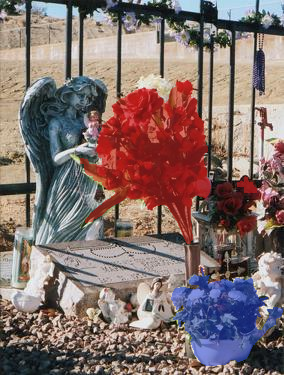
\includegraphics[height=3.5cm,width=\linewidth,keepaspectratio]{figures/pascal_total_miss.png}
    \caption{}
    \label{fig:pascal-total-miss}
\end{subfigure}
\hfill
\begin{subfigure}[b]{0.48\linewidth}
    \centering
    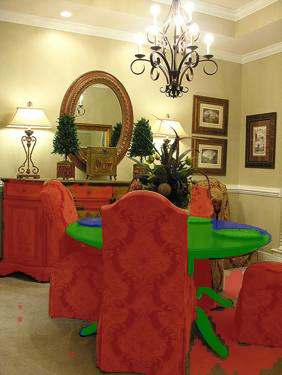
\includegraphics[height=3.5cm,width=\linewidth,keepaspectratio]{figures/pascal_oversegmentation.png}
    \caption{}
    \label{fig:pascal-overseg}
\end{subfigure}
\caption{Representative PASCAL-VOC failure cases (TP=green, FP=red, FN=blue). (a) A total-miss case (pottedplant, image \texttt{img\_1005}): the pipeline segments a large red flower bouquet in the scene, while the annotated ground-truth object -- a small blue potted plant -- remains unmarked, suggesting object-identity confusion among multiple plausible candidates rather than an outright failure to detect any plant-like structure. (b) A classic over-segmentation case (diningtable, image \texttt{img\_1014}): the table is correctly localized (green) but the predicted region extends well beyond its boundary (red), consistent with the graded over-segmentation pattern discussed in the text.}
\label{fig:pascal-failure-modes}
\end{figure}

\paragraph{Within-class variance, not a subgroup structure, is the relevant heterogeneity signal.} Unlike iCoseg, PASCAL-VOC's 20 classes are atomic categories without the multi-subgroup structure that motivated the intra-family analysis above; the comparable evidence against per-class tuning here instead comes from within-class IoU variance ($\text{iou\_std}$) across the individual images of each class. This variance correlates only weakly with class-level mean IoU ($r=-0.190$), meaning low performance and high inconsistency are largely independent phenomena. Some low-performing classes are consistently weak: diningtable has both a low mean IoU (0.267) and one of the lowest within-class spreads (iou\_std $=0.178$), indicating uniformly poor performance across its 14 images rather than a few outliers dragging down the average. Others show the opposite pattern: bottle reaches a moderate mean IoU (0.539) despite the highest within-class spread in the dataset (iou\_std $=0.389$, nearly as large as the mean itself), implying its 44 images range from near-total failure to near-perfect segmentation. As on iCoseg, this heterogeneity -- whether concentrated in a uniformly hard class or scattered unpredictably within an otherwise moderate one -- offers no stable target for per-class hyperparameter tuning, reinforcing the same dual-criterion policy applied throughout this work.

\subsection{Qualitative Results}
\label{sec:qualitative}

Figure~\ref{fig:qualitative-progression} traces the pipeline through its five stages for a representative image from Kite-Margate, the strongest iCoseg-38 group (mean IoU 0.982, iou\_std 0.0045): a large panda-shaped kite photographed against sky, with a row of coastal buildings visible in the lower portion of the frame. The chosen image (IoU 0.9816, precision 0.9991, recall 0.9824) sits within 0.0001 of the group mean, avoiding a best-case cherry-pick.
\begin{figure*}[t]
\centering
\includegraphics[width=\textwidth]{figures/qualitative_progression.png}
\caption{Pipeline progression for a representative image from Kite-Margate (iCoseg-38 group with mean IoU 0.982, iou\_std 0.0045). Left to right: original image; E2B foreground-likelihood heatmap (patch-level, pre-binarization; brighter red indicates higher foreground confidence); E3 co-saliency mask; E4 SAM2-refined mask; E5 final mask (after iterative refinement); comparison against ground truth (TP=green, FP=red, FN=blue). Per-stage foreground coverage: E3~46.0\%, E4~43.2\%, E5~53.0\%, ground truth~53.9\%. The trajectory is non-monotonic in coverage -- E4 trades area for boundary precision, and E5 recovers the loss -- despite the final result (IoU~0.9816) closely matching ground truth.}
\label{fig:qualitative-progression}
\end{figure*}

The E2B stage (panel 2) assigns high foreground likelihood broadly across the kite's silhouette, though with substantial patch-level noise -- consistent with the coarse $37{\times}37$ patch grid at this stage. E3 co-saliency (panel 3) converts this into a binary estimate covering 46.0\% of the image, already close to the ground-truth foreground fraction of 53.9\% but with visible fragmentation concentrated in the kite's lower-left region. SAM2 refinement (panel 4, E4) sharpens the object's contour but, in this instance, reduces total coverage to 43.2\% -- a step backward in area, though the resulting boundary is visibly cleaner than E3's. The iterative refinement stage (panel 5, E5) recovers and exceeds this loss, reaching 53.0\% coverage, within one percentage point of the ground truth, and produces the mask ultimately compared against ground truth in the final panel. This non-monotonic trajectory -- E3 slightly under-covers, E4 over-corrects toward precision at the expense of area, E5 recovers the balance -- illustrates that the pipeline's stages are not purely incremental refinements in the same direction; each stage corrects a different failure mode of the one before it, which is consistent with the near-perfect final result (IoU 0.9816) despite no single intermediate stage matching ground truth on its own.

\subsection{Failure Case Analysis}
\label{sec:failure-analysis}

The per-class analyses in Section~\ref{sec:per-class} identified five qualitatively distinct failure signatures across the two protocols, established with varying levels of evidence. Table~\ref{tab:failure-taxonomy} summarizes them for reference, rather than re-deriving them here.
\begin{table}[t]
\centering
\caption{Taxonomy of failure signatures identified across both protocols. Evidence level indicates how each signature was established: \emph{per-image confirmed} means verified directly from per-image precision/recall/IoU across the full class or subgroup; \emph{single case} means illustrated by one manually-inspected representative image, not systematically verified across the class; \emph{aggregate heuristic} means inferred only from class-level precision-recall gap, not confirmed at the per-image level.}
\label{tab:failure-taxonomy}
\begin{tabular}{p{2.1cm}p{2.3cm}p{1.5cm}p{1.2cm}}
\toprule
Signature & Where observed & Evidence level & Ref. \\
\midrule
Bimodal collapse & Airshows-planes (61.5\%), Huntsville (27.3\%); pottedplant (36.6\%), chair (33.3\%), person (20.9\%) & Per-image confirmed & \ref{sec:per-class-icoseg}, \ref{sec:per-class-pascal} \\
\addlinespace
Graded over-segmentation & Airshows-helicopter; most of the ten lowest-IoU iCoseg groups; diningtable, bicycle & Per-image confirmed & \ref{sec:per-class-icoseg}, \ref{sec:per-class-pascal} \\
\addlinespace
Object-identity confusion & pottedplant (image \texttt{img\_1005}; does not generalize to the class's other 14 total misses) & Single case, non-generalizing & \ref{sec:per-class-pascal}, \ref{sec:failure-analysis} \\
\addlinespace
Under-segmentation & Monks (iCoseg); confirmed in 15/17 images & Per-image confirmed & \ref{sec:per-class-icoseg}, \ref{sec:failure-analysis} \\
\addlinespace
Unresolved / ambiguous & Windmill, Kite-Brighton (iCoseg) & Aggregate heuristic, inconclusive & \ref{sec:per-class-icoseg} \\
\bottomrule
\end{tabular}
\end{table}

Two of these five rows warrant an explicit note. First, \emph{object-identity confusion} was observed in a single representative case (img\_1005), motivating a check of whether the same mechanism -- a second, visually distinct plant-like object competing for the shared-object role -- explains pottedplant's other 14 total misses. Direct inspection of all 15 total-miss images (not included as a figure due to space) shows that it does not generalize: the false-positive region in the remaining 14 images corresponds to 14 different objects unrelated to plants (e.g., a cat, a window frame, a chair, a bicycle, a dining set), with no shared visual category, texture, or structural property across cases.Three of these five rows warrant an explicit note. First, \emph{object-identity confusion} was observed in a single representative case (img\_1005), motivating a check of whether the same mechanism -- a second, visually distinct plant-like object competing for the shared-object role -- explains pottedplant's other 14 total misses. Direct inspection of all 15 total-miss images (not included as a figure due to space) shows that it does not generalize: the false-positive region in the remaining 14 images corresponds to 14 different objects unrelated to plants (e.g., a cat, a window frame, a chair, a bicycle, a dining set), with no shared visual category, texture, or structural property across cases. One partial statistical driver does emerge, however: total-miss images have their ground-truth object positioned, on average, substantially farther from the image center than successful images (mean normalized centroid distance 0.393 vs.\ 0.241), and centrality distance correlates moderately with IoU across all 41 pottedplant images ($r=-0.486$). This is consistent with a centrality bias in the pipeline's saliency scoring (Section~\ref{sec:e3-graph} notes that cluster selection incorporates a centrality term), though the effect is neither universal nor sufficient on its own: two total misses have highly centered objects (\texttt{img\_1037}, \texttt{img\_1028}, both under 0.07 normalized distance), and two peripheral objects (\texttt{img\_1021}, \texttt{img\_1041}, both above 0.39) still achieve moderate IoU (0.576 and 0.492, respectively). Unlike the bimodal and over-segmentation signatures, which share one mechanism across many images, pottedplant's total misses therefore appear to be driven by a combination of a moderate centrality bias and pairwise correspondence errors specific to each image pair, rather than a single identifiable failure mode; fully isolating and quantifying each contributing factor is left to an extended version of this work.

Second, per-image inspection of Monks (17 images) confirms the under-segmentation signature suggested by the aggregate gap: 15 of 17 images show precision exceeding recall, with the gap exceeding $+0.15$ in five cases; one image is a total miss (\texttt{2619130048}), and only one shows the opposite direction, with recall modestly exceeding precision while still achieving a good result (IoU 0.807). The remaining seven images are near-perfect (IoU~$>0.96$), indicating that Monks' moderate aggregate IoU (0.634) reflects a genuinely under-segmenting minority rather than uniformly mediocre performance across the class.

Third, the \emph{unresolved} row (Windmill, Kite-Brighton) was never confirmed by per-image inspection, unlike the other four signatures in Table~\ref{tab:failure-taxonomy}; Section~\ref{sec:per-class-icoseg} already notes that the gap-based heuristic used to assign these labels cannot rule out a bimodal pattern for these two groups.

\paragraph{Extending the color-uniformity analysis to PASCAL-VOC.} Section~\ref{sec:per-class-pascal} left open whether the false-positive color-uniformity signature established for Airshows (Section~\ref{sec:per-class-icoseg}: lower color variance inside false-positive regions than inside the true foreground, in 63 of 73 images) also holds for the bimodal PASCAL classes. We do not pursue this extension. The mechanism motivating the original test -- a single large, visually uniform background structure (sky, cloud, haze) competing with a small foreground object -- is characteristic of Airshows' outdoor, sky-dominated scenes, but not obviously applicable to PASCAL-VOC's indoor and urban clutter, where multiple visually heterogeneous objects typically share the frame. Consistent with this, none of the 15 pottedplant total-miss cases directly inspected above fit the uniform-background pattern: false positives corresponded to 14 different, visually heterogeneous objects (a flower bouquet, a cat, a window frame, a chair, among others), never a flat or uniform region, and the dominant statistical driver identified instead -- object centrality -- is unrelated to background uniformity altogether. This suggests that a color-uniformity test calibrated for Airshows would likely not transfer to PASCAL's failure mode without modification, making a direct extension both costly and of uncertain value; we leave a PASCAL-specific formulation of this analysis, if warranted, to future work.

% Optional
%\subsection{Computational Performance}
%\label{sec:computational-performance}

\section{Ablation Studies}
\label{sec:ablation}
\label{sec:ablation-backbone}

\section{Discussion}
An interesting direction for future work is inter-class co-segmentation, where semantically related but visually distinct object categories (e.g., car--bus--train) must be jointly segmented within the same image set. Amir et al.~\cite{amir2022deepvit} introduce PASCAL-CO specifically for this setting and show that dense ViT features generalize surprisingly well across related categories. Our current pipeline is not designed for this scenario: the \texttt{semantic} protocol's \texttt{CLASS\_GROUP\_OVERRIDES} mechanism merges subgroups that are assumed to share the same underlying object category (e.g., different Panda image sets), rather than reasoning across genuinely distinct classes. Extending the correspondence and co-saliency stages (E2--E3) to support cross-class grouping would be a natural next step, though it would likely require revisiting the spatial saliency prior and the FG/BG decision heuristic, both of which implicitly assume a single dominant object category per collection.

\section{Conclusion}
\input{sections/08_conclusion}

% -----------------------------------------------------------------------------
% Acknowledgments
% -----------------------------------------------------------------------------
% Uncomment when needed.
%
% \section*{Acknowledgment}
% The authors would like to thank ...

% -----------------------------------------------------------------------------
% References
% -----------------------------------------------------------------------------
% During the initial drafting stage, \nocite{*} allows BibTeX to compile even
% before explicit citations are added. Remove \nocite{*} before submission so
% that only cited references appear in the bibliography.
\bibliographystyle{IEEEtran}
\bibliography{references}

\end{document}
